\documentclass[11.5pt]{sig-alternate} % sets document style to sig-alternate
% packages
% typesetting
%\usepackage{dirtytalk} % typset quotations easier (\say{stuff})
\usepackage{hanging} % hanging paragraphs
\usepackage[defaultlines=3,all]{nowidow} % avoid widows
\usepackage[pdfpagelabels=false]{hyperref} % produce hypertext links, includes backref and nameref
\usepackage{xurl} % defines url linebreaks, loads url package
\usepackage{microtype}
\usepackage{textgreek}
\usepackage{pdfpages}
%\usepackage{textcomp}
%\newcommand{\texttildemid}{\raisebox{0.4ex}{\texttildelow}}
% layout
\usepackage{enumitem} % control layout of itemize, enumerate, description
\usepackage{fancyhdr} % control page headers and footers
\usepackage{float} % improved interface for floating objects
%\usepackage{multicol} % intermix single and multiple column pages
% language
\usepackage[utf8]{inputenc} % accept different input encodings
\usepackage[english]{babel} % multilanguage support
% misc
\usepackage{graphicx} % builds upon graphics package, \includegraphics
%\usepackage{lastpage} % reference number of pages
%\usepackage{comment} % exclude portions of text (?)
\usepackage{xcolor} % color extensions
\usepackage[backend=biber, style=apa]{biblatex} % sophisticated bibliographies % necessary for HTML to display author info and date on abstract page
\usepackage{csquotes} % advanced quotations, makes biblatex happy
\usepackage{authblk} % support for footnote style author/affiliation
% tables and figures
\usepackage{tabularray}
\UseTblrLibrary{varwidth}
%\usepackage{array} % extend array and tabular environments
\usepackage{caption} % customize captions in figures and tables (rotating captions, sideways captions, etc)
%\usepackage{cuted} % allow mixing of \onecolumn and \twocolumn on same page
\usepackage{multirow} % create tabular cells spanning multiple rows
%\usepackage{subfigure} % deprecated, support for manipulation of small figures
%\usepackage{tabularx} % extension of tabular with column designator "x", creates paragraph-like column whose width automatically expands
%\usepackage{wrapfig} % allows figures or tables to have text wrapped around them
%\usepackage{booktabs} % better rules
% dummy text
%\usepackage{blindtext} % blind text dummy text
%\usepackage{kantlipsum} % Kant style dummy text
\usepackage{lipsum} %lorem ipsum dummy text
% other helpful packages may be booktabs, longtable, longtabu, microtype

\pagestyle{fancy} % sets pagestyle to fancy for fancy headers and footers

% header and footer
% modern way to set header image
\renewcommand{\headrulewidth}{0pt} % defines thickness of line under header
\renewcommand{\footrulewidth}{0pt} % defines thickness of line above header
\setlength\headheight{80.0pt} % sets height between top margin and header image, effectively moves page contents down
\addtolength{\textheight}{-80.0pt} % seems to affect the lower height. maybe only works properly if footer numbers enabled?
\fancyhf{}
\fancyhead[CE, CO]{
\includegraphics[width=\textwidth]{headerImage.png}}
% footer
%\fancyfoot[LE,LO]{Article Title Here \\ DOI: }% left footer article title and doi
%\fancyfoot[CE,CO]{{}} % center footer empty
%\fancyfoot[RE,RO]{\thepage} % right footer page numbers
%\pagenumbering{arabic} % arabic (1, 2, 3) numbering in footer

\hypersetup{colorlinks=true,urlcolor=blue} % sets link color to blue
\urlstyle{same} % sets url typeface to same as rest of text

% set caption and figure to italics, label bold, left align captions, does not transfer to HTML
\captionsetup{labelfont=bf, font={large, it}, justification=raggedright, singlelinecheck=false}
\renewcommand\theContinuedFloat{\alph{ContinuedFloat}}

%this next bit is confusing, but essentially changes the width of the abstract. Seems to have been copied from this https://tex.stackexchange.com/questions/151583/how-to-adjust-the-width-of-abstract
\let\oldabstract\abstract
\let\oldendabstract\endabstract
\makeatletter %changes @ catcode to enable modification (in parsep)
\renewenvironment{abstract} %alters the abstract environment
{\renewenvironment{quotation}%
               {\list{}{\addtolength{\leftmargin}{1em} % change this value to add or remove length to the the default ?
                        \listparindent 1.5em%
                        \itemindent    \listparindent%
                        \rightmargin   \leftmargin%
                        \parsep        \z@ \@plus\p@}%
                \item\relax}%
               {\endlist}%
\oldabstract}
{\oldendabstract}
\makeatother %changes @ catcode to disable modification

% checks
% italics -
% links -
% dashes -
% tildes -
\begin{document}

\title{Pre-College Deaf Students’ Understanding of Fractional Concepts: What We Know and What We Do Not Know}

\author[1]{\large \color{blue}Keith Mousley}
\author[1]{\large \color{blue}Christopher Kurz}

\affil[1]{Rochester Institute of Technology}

\toappear{}
%% ABSTRACT
\maketitle
\begin{@twocolumnfalse} 
\begin{abstract}
\item 
\textit{Mathematical knowledge and skills are crucial to success in academics and the workplace. The Common Core State Standards emphasizes fraction teaching and learning in elementary school. This mixed-method study explores fraction concept understanding among 14 deaf and hard of hearing participants between the ages of 8 and 16, as quantitatively measured by their ability to describe the properties of fractional numbers, convert between fractional numbers and their visual representations, and determine the order and equivalence of fractional numbers. Furthermore, the qualitative study was supplemented by interviews with the deaf participants and surveys with their parents and teachers to examine use of mathematical fraction concepts in the student participant's experience, at home and in the classroom. Results indicated a strong understanding of fractional magnitude; however, putting fractions in order from the smallest to the largest was a struggle for the participants. The findings also support the call for increased incidental learning opportunities between deaf and hard of hearing children and their parents along with increased use of practical applications of fractional numbers, and additional training for teachers who teach fractions to deaf students.}
\\ \\
Keywords: Science Education, Deaf Education, American Sign Language, Direct Communication, Educational Interpreter
\end{abstract}
\end{@twocolumnfalse}

%% AUTHOR INFORMATION

\textbf{*Corresponding Author, Keith Mousley}\\
\href{mailto: kxmntm@rit.edu }{(kxmntm@rit.edu)} \\
\textit{Submitted  Dec 3 2015 }\\
\textit{Accepted Jan 21 2016} \\
\textit{Published online Feb 22 2016} \\
\textit{DOI: 10.14448/jsesd.07.0004} \\
\pagebreak
\clearpage
\begin{large}
\section*{INTRODUCTION}

Researchers and practitioners know that mathematics is not just adding and subtracting. Fractions are used by individuals daily in typical life processes. Lesh, Post, \& Behr (1988) “believe proportional reasoning is both the capstone of elementary arithmetic and the cornerstone of all that is to follow. It therefore occupies a pivotal position in school mathematics (and science) programs.” 

The manner in which fractions are worded in everyday English sentences can be complex and sometimes confusing to students.  In fact, the English language itself has so many comparisons and relationships, and the challenge is: Do our students keep up with the dialogue of mathematics? There are very few research articles on teaching fractions in the field of deaf education. Because of the lack of research done to date on the topic, the authors are determined to investigate deaf students’ knowledge and learning of fractions. Both of the authors are mathematics professors at the college level and continue to see a lack of skill in the area of fractions. According to Bone, et al. (1984) the Model Secondary School for the Deaf and the National Technical Institute for the Deaf have noted specific deficiencies in understanding by post-secondary deaf and hard of hearing students— including knowledge of rational number topics such as fractions.

The authors have been investigating the important role of fractions in the mathematics curriculum for the past decade. The authors’ interest in this topic stems from their own experiences teaching in the classroom and from on-going community dialogues among other math teachers for the deaf. These dialogues represented a series of discussions that led to requests for more information regarding fraction learning. The authors met to discuss their experiences teaching mathematics and to share the frustrations of college students trying to learn various topics in Algebra.  Among the common reactions deaf students had when learning fractions were: “\textit{I hate fractions}”, “\textit{I don’t understand fractions}”, “\textit{Do we need to use fractions?}” and “\textit{Can we avoid fractions?}”

Research by Siegler, R. S., Thompson, C. A., \& Schneider, M (2011) shows that “early knowledge in [fraction and long division] were absolutely crucial to later learning of more advanced mathematics, but did not have any evidence until now.” Additionally, “understanding fractions is central to subsequent mathematics learning, [and] early knowledge of fractions is highly predictive of much later mathematics achievement” (Bailey, D. H., et.al, 2014). Given that having a basic understanding of fractions is a crucial building block of learning mathematics, it seems prudent to revisit the fraction curriculum and to make some recommendations for improvement. 

According to the National Council of Teachers of Mathematics, instruction of fractions begins early in a child’s schooling. In first grade, students are expected to become familiar with basic fraction knowledge and understand the part and whole concept for fractions as well as basic operations (NCTM, 1989). The Council suggests, during that process, students have a dialogue about fractions in general as well as their application in real-life. Students should investigate possible applications of basic fractions in various settings (NCTM, 1989). Later in school, especially from fourth to sixth grade, students learn how to do operations with fractions. More proportional reasoning and problem-solving situations are introduced as students form the foundations for later topics in mathematics. Fractions are then expected to be used and be taught in higher mathematics from elementary to high school (NCTM, 1989).

To increase rigor and standardize mathematical learning, the National Council of Teachers of Mathematics (NCTM) proposed standards for mathematical literacy including conceptual understanding of mathematics, problem solving, communicating mathematics, and reasoning at all levels of the curriculum (NCTM, 1989). After several attempts in standardizing mathematics education during the past two decades, states across the country are now adopting new standards, the Common Core State Standards (CCSS). The CCSS were developed and published in 2010 by the National Governors Association Center for Best Practices (NGACBP) to increase rigor and relevance of mathematics and English language arts for students. Instruction of fractions, according to the CCSS for mathematics, begins early in school. Starting in third grade, students are expected to develop an understanding of fractions as numbers, beginning with unit fractions (NGACBP, 2010). Unit fractions are basic units of measurement in fractions of which fractions in general are built out. Common unit fractions for third graders are 1/2, 1/3, and 1/5. Students are expected to understand that “the size of a fractional part is relative to the size of the whole” and to compare fractions to represent numbers equal to, less than, and greater than one (NGACBP, 2010). As the CCSS suggest, during that process, students have a dialogue about fractions and their application in real-life and investigate possible applications of basic fractions in various settings.  Later in school, especially in fourth grade, students learn fraction equivalence, are able to put fractions in order in terms of size, and do operations (addition, subtraction, multiplication and division) with fractions (NGACBP, 2010).  For the state of New York Common Core, the total number of days spent on fractions from third to fifth grade is 215 days.  For third grade, instructors focus where on the number line fractions go for 35 days (New York State Department of Education, 2010).Whether this amount of time devoted to fractions, especially for students who may struggle with the language in the writing of the mathematical problems, is sufficient enough would be appropriate for curriculum committees to consider.

The understanding and applications of fractions are basic mathematical skills required by everyone (Markey, et al., 2003). Experienced mathematics educators want to understand why students in general are having trouble learning fractions. Below is an excerpt from Runde (2015), a collector of math jokes.			


\begin{quote}
\textit{The Chef instructs his apprentice: “You take two thirds of water, one third of cream, one third of broth…” The Apprentice: “BUT that makes four thirds already!” Chef: “Well – just take a larger pot!”}
\end{quote}

So what is it that makes fractions so difficult to learn? For one, many teachers find fractions as a topic that is difficult to teach (Clarke, Roche, Mitchell, and Sukenik, 2006, Ma, 1999). There is a consensus among educational researchers that the difficulties of teaching and learning are tied to the fact that fractions include a multifaceted construct (Brousseau, Brousseau \& Warfield, 2004, Lamon, 2001).  Behr, Lesh, Post, and Silver (1993) categorized interpretations of fractions into five sub-constructs: Part-whole, quotient, ratio, operator (division), and measure. This study is primarily focused on two areas: 1) the magnitude of the fraction and 2) adding and/or subtracting fractions. Not understanding the size of the fraction can lead to it being more difficult for the student to grasp the concept of fractions in general, which includes the ability to add/subtract fractions. 

The number of interpretations may make it difficult to fully understand (Kilpatrick, Swafford, \& Findell, 2001); but students’ difficulty in learning fractions has many sources, with erroneous assumptions that properties of whole numbers are properties of all numbers and relations among arithmetic procedures being two of the most significant ones (Siegler, R. S., Thompson, C. A., \& Schneider, M, 2011). In another research project, whole number knowledge and fraction knowledge were found to be interconnected; if a person has a good knowledge of whole numbers, chances are that this person will also have a good knowledge of fractions (Siegler, Fazio, Bailey, \& Zhou, 2013).  

Research shows a deficiency in mathematical knowledge when deaf and hard of hearing children enter school. There is a lag in deaf students’ achievement in mathematics: basic mathematical concepts (Kritzer, 2009), number sequence (Leybart \& VanCustem, 2002), relationship representation (Blatto-Valle, Kelly \& Gaustad, 2007), mathematics computations (Traxler, 2000), and problem solving (Qi \& Mitchell, 2007). Knowledge in these areas is crucial to a conceptual understanding of mathematics. Two significant factors that have created this delay are: lack of early exposure to basic mathematical concepts (Kritzer, 2009), and lack of teacher training in specialized content area, especially in mathematics (Pagliaro, 1998 and Lang and Pagliaro, 2007)). 

Marschark and Everhart (1999) found that students have difficulty in tasks involving logical thinking, and Allen (1995) found that students have difficulty in tasks involving reasoning. Zar\-faty, Nunes, and Bryant (2004) found that deaf children's mathematics ability for representing numbers was at least as good as their hearing peers. Multiple suggestions are offered to make a change in the teaching of fractions. Silva (1986) noted the difficulty of teaching fractions to deaf students, which led to her to try a new approach. Silva tried to substitute some of the complexity by using gzorkes, fattening, reducing, making trades, etc. to help reduce the confusion of fraction operations. Silva’s strategy involves having a deep, thought provoking discussion about what fractions are and how fractions are being used. However, to effectively use this approach, the instructor must have good signing skills. To this end, Lang and Pagliaro (2007) reported that a teacher's usage of sign language in math classes could influence the content knowledge of the students.

There are numerous studies examining the effects of English on mathematical learning (Hyde et al., 2003: Kelly \& Mousley, 2001: Kelly, Lang, Mousley, \& Davis, 2003; Kidd \& Lamb, 1993; Kidd, Madsen, \& Lamb, 1993). The authors have reported that the following variables have been known to cause some level of hindrance to deaf or hard of hearing students’ ability to learn mathematical concepts: use of conditionals, comparatives, negatives and inferential.
 
One research study discussed the use of rote memorization when teaching mathematics, such as using multiplication drills, and the use of flash cards for addition, subtraction, and division (Paul, 2012). Paul (2012) shared that math educators should encourage students to do math drills over again and again in order to help them improve student math skills. The same study also revealed that educators noticed that there are significant differences in the math scores of American and Chinese students on international tests (Paul, 2012). This was attributed to the fact that the Chinese students’ schools’ philosophy focused on math drills and on memorizing math facts. Another research study found that many errors made by students working on complex math problems were due to an inability to understanding of how to apply basic math facts (Cumming \& Elkins, 2010).

After a review of the literature, the authors found that there is a paucity of materials related specifically to best practices for teaching fractions to deaf students. The purpose of the following study is to expand the amount of information available about the difficulties of deaf students in the area of fractions. Furthermore, the authors explore the development and comprehension of fractional concepts in deaf children and identify factors that promote such development and understanding of fractional concepts.

In this study, the authors set out to investigate the following fundamental research questions related to student understanding and learning of fractions:

 \begin{enumerate}
     \item Is there a relationship between measures that examine concept/ magnitude, order, and equivalence of fractions (written test and interview)?
     \item Is there a difference in scores on fraction test between the demographic variables (school settings, parent’s educational attainment, and representations)?
     \item In which representation(s) do deaf participants understand fractional numbers the best? Are deaf students able to describe fractional numbers in different representations (e.g., numbers and illustrations)? In other words, do they have the ability to translate fractional numbers into pictures, and vice versa?
 \end{enumerate}
 
\section*{METHODS}

This mixed-method research study includes participant videotaped interviews, paper tests, and parent surveys. An example of the paper test can be found in the Appendix. A more detailed discussion of the parent survey will be included in a forthcoming article by the authors.

\subsection*{Instruments:}

The \textbf{Student Fraction Test} includes 20 question items in three parts (concept/magnitude, order, and equivalence). The purpose of the test is to evaluate knowledge of fraction sizes, order fractions with like and unlike denominators, and fraction equivalents. The problems are presented either in text or picture formats. Below are two examples of magnitude problems in the picture format: 

\begin{figure}[h]
     \centering
     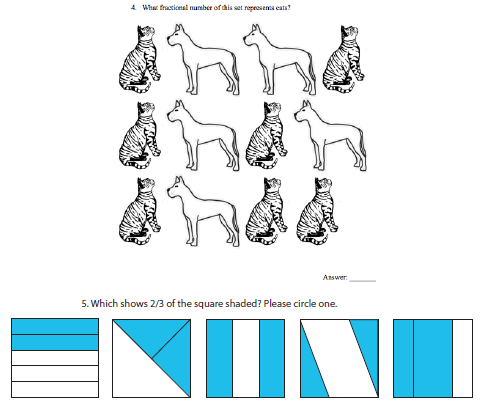
\includegraphics[width=1\linewidth]{figure1.png}
     \caption{}
 \end{figure}

An example of a problem presented in written text is:

3. 5/3 or 3/5 \hspace{0.5em} Are they equal? \hspace{0.5em} \textbf{YES} \hspace{0.5em} \textbf{NO} \hspace{0.5em} If not, which one is smaller?


The \textbf{Student Interview} includes 30 questions with follow-up probing questions for explanation and clarity. The first eleven questions focus on participant’s school background, disposition towards mathematics and fractions, and general understanding of fraction properties. During the middle of the interview, participants were asked to solve 15 fraction problems in writing or signs, in terms of magnitude, order, and equivalence. The participants were also given four story problems in text and signs and asked to solve the problems. Below is one story problem example:

\begin{quote}
\textit{Four children want to share three candy bars so that each child gets the same amount. Show how much one child can have.}
\end{quote}

The last three questions of the survey focus on participants’ experience using mathematics and fractions outside the classroom, including in the home.

There is also a two-page, written \textbf{Parent Survey} that consists of 20 questions regarding parent educational and communication background, disposition towards mathematics, and use of mathematics at home.

\subsection*{Procedure:}

The researchers contacted schools for the deaf, public schools, and parents for possible testing of this study. Once deaf children, ages 8 to 16, were identified, permission was secured from them and their parents. The demographics of the deaf student participants can be found in Table 1. The participants were interviewed by one of the two authors (or both) in their selected settings. Beside background questions, the interview included some fractional number problems, in which the participant was asked to find a fractional number to represent the given image, to find the correct image to match the given fractional number, to find equivalent fractions for a given fraction, and to arrange fractional numbers in order of magnitude. In the half-hour interview, the participants discussed their thoughts and understanding of fractional numbers and their answers to fraction problems. The interview was videotaped for the purpose of documentation. After the interview, they took the test on fractions. The test covered similar problems that are shown during the interview. The interview and the test altogether took approximately 60 minutes. A total of 14 deaf and hard of hearing children participated in the interview and took the test individually. The tests were scored quantitatively by an independent eduacator with a mathematics background. The videos of interviews were also assessed by the authors, with some of the quantitative findings discussed below. A qualitative assessment of the interviews are the basis of a forthcoming article.

\begin{table}[ht]
\caption{Demographics of Student Participants}
\begin{tabular}{|l|c|c|}
\hline
Characteristics & N & \% \\ \hline
Age Ranges & & \\
\begin{itemize}[noitemsep, topsep=0pt] \item 8-10 \end{itemize} & 3 & 21.4\% \\
\begin{itemize}[noitemsep, topsep=0pt] \item 11-13 \end{itemize} & 9 & 64.3\% \\
\begin{itemize}[noitemsep, topsep=0pt] \item 13-16 \end{itemize} & 2 & 14.3\% \\ \hline
Grade Ranges & & \\
\begin{itemize}[noitemsep, topsep=0pt] \item 2-4 \end{itemize} & 2 & 14.3\% \\
\begin{itemize}[noitemsep, topsep=0pt] \item 5-7 \end{itemize} & 8 & 57.1\% \\
\begin{itemize}[noitemsep, topsep=0pt] \item 13-16 \end{itemize} & 4 & 28.6\% \\ \hline
School Settings & & \\
\begin{itemize}[noitemsep, topsep=0pt] \item School for the deaf \end{itemize} & 5 & 35.7\% \\
\begin{itemize}[noitemsep, topsep=0pt] \item Mainstreamed \end{itemize} & 9 & 64.3\% \\ \hline
Parents' Hearing Status & & \\
\begin{itemize}[noitemsep, topsep=0pt] \item Both Deaf \end{itemize} & 4 & 28.6\% \\
\begin{itemize}[noitemsep, topsep=0pt] \item One Deaf/One Hearing \end{itemize} & 3 & 21.4\% \\
\begin{itemize}[noitemsep, topsep=0pt] \item Both Hearing \end{itemize} & 5 & 35.7\% \\
\begin{itemize}[noitemsep, topsep=0pt] \item N/A \end{itemize} & 1 & 7.3\% \\ \hline
Deaf Siblings & & \\
\begin{itemize}[noitemsep, topsep=0pt] \item Yes \end{itemize} & 4 & 28.6\% \\
\begin{itemize}[noitemsep, topsep=0pt] \item No \end{itemize} & 10 & 71.4\% \\ \hline
\end{tabular}
\end{table}

A written survey was sent to the participant's parent(s) with a self-addressed, pre-stamped envelope for return. This survey asked them questions about their demographics (hearing status, educational background, communication use, signing skills, deaf sibling) and use of fractions at home. The parental responses allowed the researchers to learn more about daily use of mathematics, especially fractional numbers, at home among parents and their deaf and hard of hearing children. The survey took approximately 15 minutes to complete. A total of 14 parents participated in the survey. Demographics of Participant's Parents can be found in Table 2.

\begin{table}[htbp]
\caption{Demographics of Participant's Parents}
\begin{tabular}{|l|c|}
\hline
Mother's Hearing Status & \\
\begin{itemize}[noitemsep, topsep=0pt] \item Deaf \end{itemize} & 3 \\
\begin{itemize}[noitemsep, topsep=0pt] \item Hard of Hearing \end{itemize} & 1 \\
\begin{itemize}[noitemsep, topsep=0pt] \item Hearing \end{itemize} & 5 \\
\begin{itemize}[noitemsep, topsep=0pt] \item N/A \end{itemize} & 1 \\ \hline
Father's Hearing Status & \\
\begin{itemize}[noitemsep, topsep=0pt] \item Deaf \end{itemize} & 5 \\
\begin{itemize}[noitemsep, topsep=0pt] \item Hearing \end{itemize} & 8 \\
\begin{itemize}[noitemsep, topsep=0pt] \item N/A \end{itemize} & 1 \\ \hline
Mother's Highest Educational Attainment & \\
\begin{itemize}[noitemsep, topsep=0pt] \item Grade 8 \end{itemize} & 1 \\
\begin{itemize}[noitemsep, topsep=0pt] \item High School \end{itemize} & 2 \\
\begin{itemize}[noitemsep, topsep=0pt] \item Some College \end{itemize} & 2 \\
\begin{itemize}[noitemsep, topsep=0pt] \item Associate’s Degree \end{itemize} & 1 \\
\begin{itemize}[noitemsep, topsep=0pt] \item Bachelor’s Degree \end{itemize} & 2 \\
\begin{itemize}[noitemsep, topsep=0pt] \item Master’s Degree \end{itemize} & 5 \\
\begin{itemize}[noitemsep, topsep=0pt] \item N/A \end{itemize} & 1 \\ \hline
Father's Highest Educational Attainment & \\
\begin{itemize}[noitemsep, topsep=0pt] \item Grade 8 \end{itemize} & 1 \\
\begin{itemize}[noitemsep, topsep=0pt] \item High School \end{itemize} & 4 \\
\begin{itemize}[noitemsep, topsep=0pt] \item Associate's Degree \end{itemize} & 0 \\
\begin{itemize}[noitemsep, topsep=0pt] \item Bachelor's Degree \end{itemize} & 2 \\
\begin{itemize}[noitemsep, topsep=0pt] \item Master's Degree \end{itemize} & 5 \\
\begin{itemize}[noitemsep, topsep=0pt] \item N/A \end{itemize} & 2 \\ \hline
Communication at Home & \\
\begin{itemize}[noitemsep, topsep=0pt] \item Signing alone \end{itemize} & 5 \\
\begin{itemize}[noitemsep, topsep=0pt] \item Voice and signing all the time \end{itemize} & 3 \\
\begin{itemize}[noitemsep, topsep=0pt] \item Voice and some signs and fingerspelling \end{itemize} & 3 \\
\begin{itemize}[noitemsep, topsep=0pt] \item Using voice only \end{itemize} & 3 \\ \hline
Self-Rating Signing Skills & \\
\begin{itemize}[noitemsep, topsep=0pt] \item 1 little knowledge \end{itemize} & 3 \\
\begin{itemize}[noitemsep, topsep=0pt] \item 2 \end{itemize} & 3 \\
\begin{itemize}[noitemsep, topsep=0pt] \item 3 \end{itemize} & 2 \\
\begin{itemize}[noitemsep, topsep=0pt] \item 4 \end{itemize} & 4 \\
\begin{itemize}[noitemsep, topsep=0pt] \item 5 Fluency \end{itemize} & 2 \\ \hline
\end{tabular}
\end{table}

\subsection*{Demographics:}

The demographics of the participants and their parents in this study are shown in Tables 1 and 2, respectively. The students in the study self-identified themselves as being deaf or hard of hearing. Likewise, parents self-identified themselves as being hearing, deaf, or hard of hearing. We did not assess whether individuals used hearing aids, cochlear implants, etc. nor their level of hearing loss and age of onset. These characteristics were beyond the scope of this study. Likewise, the socioeconomic status and standardized test scores were not included as part of this study, but all would be good characteristics to examine in future studies. Students who attended the schools for the deaf were all commuters involved in day programs. The mainstreamed students were deaf or hard of hearing students enrolled in hearing schools, and may have taken their mathematics courses in self-contained or fully integrated classes.

\section*{RESULTS}

\textit{Written Test Results: Magnitude, Order and Equivalence Competence}

A summary of results from the student written tests is shown in Table 3. The mean of the written test (n=14) is 48.4\% with the standard deviation of 21.9\%. The range of the test is from 17\% to 83\%. Due to limitations of sample sizes in this study, it was not feasible to do detailed quantitative analyses, like ANOVA tests. Future studies, with larger sample sizes, would be greatly beneficial to the field. It is interesting though that there were not large differences between the scores of when students were given questions with words and when they were given questions with pictures.

\begin{table}[ht]
\caption{Students’ written test (number of correct answers compared to total number of questions)}
\begin{tabular}{|l|c|c|c|}
\hline
 & Concept/ Magnitude & Equivalence & Fraction in Order \\ \hline
Questions with words: & 48\% & 57\% & 21\% \\ \hline
Questions with pictures: & 60\% & 38\% & 7\% \\ \hline
\end{tabular}
\end{table}

In the area of Concept/Magnitude, the findings are somewhat consistent for all the subjects. The common errors that were shown in this area were related to equal parts and making use of the fraction. The equal parts, for example, involved asking the subjects to draw 2/7.  Half of the subjects were able to draw the fraction accurately. The common error was the drawing of unequal parts. The other error was the use of the fraction, part over whole. If you recall the question above with cats and dogs (see Figure 1), 57\% of the subjects were able to determine the fraction accurately. The errors were that the subjects were not sure how to find the denominator.

In the area of Equivalence, 57\% of the subjects were able to answer the written questions. In Figure 1, one question with pictures asks, “which shows 2/3 of the square shaded?”  Of all the subjects, 36\% were able to find the correct answer. The errors showed that subjects had difficulty trying to figure out part over whole. The number of parts for the numerator and the numbers of parts for the denominator were confusing among the subjects.

The area of Order was difficult for most of the subjects. Sample questions include “which is smaller, 5/3 or 3/5” or “put the fractions in order from the smallest to the largest, 1/5, 3/4, 1/2”. Most of the subjects followed the size of the denominator when answering the questions. In this case, 1/2 would be declared the smallest because two is the smallest number, then 3/4 would be next, and the last would be 1/5. The results show that understanding the size of the fraction is not strength among the subjects.

Participants with deaf parents and those with hearing parents show differences in the total score on the test. The difference in total was significant (p < 0.001). Deaf subjects with deaf parents fared well in the written test across the board (magnitude– 80\%; order– 53\%, equivalence– 52\%, total– 61\%), scoring higher than those subjects with hearing parents (magnitude– 40\%; order– 48\%, equivalence– 44\%, total– 44\%). The authors are fully aware that the sample size of this study is relatively small. Further research would be needed to see if these findings are consistent.

\begin{table}[ht]
\caption{Students’ interview test}
\begin{tabular}{|l|l|}
\hline
Type of questions & Result in \% \\ \hline
Fraction Same or different & 80 \% \\ \hline
Identify Fraction Larger or smaller & 40\% \\ \hline
Ranking fraction in order: using word descriptions & 21\% \\ \hline
Ranking fraction in order: using pictures & 7\% \\ \hline
\end{tabular}
\end{table}

\subsection*{Interview Results:}

During the interviews, the authors continued a dialogue with the students. It was presumed that this more thought-provoking process would uncover clues as to how the students think about fractions. Interview results are shown in Table 4. Due to limitations of sample sizes in this study, it was not feasible to do detailed quantitative analyses, like ANOVA tests. Future studies, with larger sample sizes, would be greatly beneficial to the field. It was interesting though that sometimes the students self-corrected their answers during the interview. Also, removing the language barrier by having the authors conduct the interviews using sign language helped student participants remain more relaxed and be able to think clearly. The interview revealed four primary results: 1) Students were able to compare the given fractions and determine if the fractions were the same or different with 80\% accuracy. 2) Students were able to identify which fraction was larger or smaller with 40\% accuracy. 3) Students were able to rank fractions in order: Ranking fractions using word descriptions resulted in 21\% accuracy. Ranking fractions using pictures resulted in 7\% accuracy and lastly, 4) Students were able to determine the fraction values. For example, presented with two fractions, students determined that the value of the fraction with the larger denominator is higher. Further investigation with students showed that students’ drawings/diagrams (mostly in rectangular form) tended to become bigger as the denominator got bigger.

% table 4

\section*{DISCUSSION}

Findings in this section were related to the three research questions.

\textit{Research Question 1: Is there a relationship between measures that examine concept/magnitude, order, and equivalence of fractions (written test and interview)?}

While students took the test, the authors sat with the students and the session was videorecorded. After the students had completed each question, the authors probed to learn more about the students’ thought processes in answering the questions. During the written test and interview session, there were some interesting findings. First, students were able to compare the given fractions and determine if the fractions were the same or different with 80\% accuracy (see Table 4).  Students had difficulty identifying which fraction was larger or smaller, being able to do so with 40\% accuracy. Results further showed that students had difficulty ranking fractions in order of magnitude. Ranking fractions using word descriptions resulted in 21\% accuracy. Ranking fractions using pictures resulted in 7\% accuracy.  It is important to note that the fractions shown with pictures/diagrams/drawings had a higher level of difficulty. One popular belief is that deaf students are visual learners. The fraction test did not support this belief. During the interview, students had difficulty with fraction values. The authors noted students determined that the bigger the denominator, the higher the value of the fraction. Students perceived the numerator and the denominator as two separate entities. Further investigation showed that students' drawings/diagrams (mostly in rectangular form) became physically larger as the denominator got bigger. The authors noted that two participants, in the process of explaining how they got their answers, corrected themselves as they talked the interviewer through the problems and they ended up changing their answers.

\textit{Research Question 2: Is there a difference in scores on fraction test between the demographic variables (ages/grades, school settings, parent’s educational attainment, and family characteristics)?}

When the parental educational attainment factor was examined, two groups of deaf participants did well in the written test: 1) those with parents with Master’s degrees or higher and 2) parents with high school or less. These groups scored 61\% and 60\%, respectively. Interestingly, the other groups (with parents with Associate’s or Bachelor’s degrees) scored very low; 16\% and 29\%, respectively. When the group with parents who have educational levels of high school or less were examined closely, of the three participants, two students had both parents who are deaf. Because discussions at home likely help them understand how mathematical relationships work, these two students might have higher scores because of the communication mode used at home. As stated, further research in this topic will be needed.

\textit{Research Question 3: In which representation(s) do deaf participants understand fractional numbers the best? Are deaf students able to describe fractional numbers in different types of representations (e.g., numbers and illustrations)?}

The written test revealed several common processing issues; including part-to-whole, the size of the fraction, and the true meaning of the fraction. Regardless of which representation was given, students struggled with these fraction concepts. An example of the ratio type of fractions is this problem, which was asked during the interview: “There are twelve children going on a field trip. If one fourth of the children are girls, how many girls are going on the field trip?” There were many different answers given by the participants. The most common answer was 12 girls. Most of them had a difficult time understanding that the word “children” includes both boys and girls. The authors’ assumptions are that either a language barrier was being demonstrated, or that the mathematical problem was not being clearly communicated. 

There are numerous studies examining the effects of English on mathematical learning (Hyde et al., 2003: Kelly \& Mousley, 2001: Kelly, Lang, Mousley, \& Davis, 2003; Kidd \& Lamb, 1993; Kidd, Madsen, \& Lamb, 1993).  The authors have reported that the following variables have been known to cause some level of hindrance to deaf or hard of hearing students' ability to learn mathematical concepts: use of conditionals, comparatives, negatives and inferential (e.g. knowing boys and girls are children). The role of student English abilities may be significant in the high level mathematic aptitude of deaf and hard of hearing students. We believe that there is a relationship between these students demonstrated English and mathematics skills.

\subsection*{Overall Study Discussion}

During the course of this research study, several limitations were noted. The sample size was 14 students and 14 parents, which is relatively small. It was a challenge to find deaf and hard of hearing children between the ages of 8 and 16. In addition, it was difficult obtaining the approval from the parents to allow us to complete the assessments and interviews. To add to the challenges, there were various factors within the small sample size, with both students and parents. These factors include; varied communication modes, language and educational backgrounds of participants. For example, some of the parents’ first language was not English. There were many different kinds of responses on the assessment and during the interview. Many of these responses were related to the students’ varied education background. This led to various knowledge, skill levels, and understanding of fraction concepts. The schools where researchers did the assessments had very different mathematics curricula. 

The authors have been researching this topic for over six years. Additional issues have emerged since the research began.  Some of the research topics that merit additional investigation are: comparing learning experiences of deaf children of deaf parents and also deaf children of hearing parents, examining what parents/teachers think deaf children know about initial fraction concepts, and comparing this with what the children actually know. Lastly, future research is warranted on investigating factors that are associated with fractional number understanding in deaf children. Based on this research study, the authors have developed a list of recommendations for teachers, at the elementary school level, to use when teaching fractions. With a few minor adjustments to the curriculum, educators might see measurable improvements in students’ ability to comprehend fraction concepts.

\begin{enumerate}
     \item Strengthen each student’s understanding of whole numbers. The more familiar they are with whole numbers, the greater their chances of understanding fractions.
     \item Encourage students to do more drawing of fractions. When drawing, encourage students to be accurate and consistent when drawing the sizes of diagrams (as they should always be of similar sizes to represent the whole) before inserting the divisional lines because the whole is always the same regardless of the number of parts.
     \item Dialogue daily. When students talk about fractions, ask them what the numerator is and what the denominator is and what they represent. For example, for the fraction, 7/12, where seven boys are on a bus, a dialogue should ensue that examines what the 7 represents (number of boys), what the 12 represents (total number of students), and how many girls must there be on the bus. Further, help the students understand that 7 boys to 5 girls is a ratio, not a fraction; as fractions are always represented by the part over the whole. Ask thought-provoking questions to help the students better understand the difference between ratios and fractions.
     \item Do many drills with equivalent fractions. Later, when adding fractions, ask the students to make a trade for the same denominator. (Siliva, 1986) This is for lower grade levels.
     \item For upper grade levels, start the drill of lowest common denominator (LCD) and then practice adding/subtracting fractions.
     \item Provide assistance/training for parents and encourage parents to have a dialogue with their children on a regular basis, i.e. monthly meetings.
\end{enumerate}
 
The authors have ideas for activities for practice and continued development of fraction skills. There are many software games and internet games involving fractions for students to use. One excellent source of real-world fractions is sports (a topic that is of interest to many school-aged students): there are many statistics being used and can be displayed as fractions. These statistics can be an opportunity for discussion between students and parents/teachers. An excellent resource is the Singapore Math curriculum, which can be used for teachers and parents to teach children about fractions. Again, it is important to constantly expose children to fractions on a regular basis. 

In the area of curriculum and instruction, there are potential implications that discourage learning fractions. In the area of problem solving, the authors suggest minimizing the use of non-realistic examples in problem solving. It is recommended for the instructors to personalize word problems. Instructors are encouraged to talk about comparisons instead of relying totally on diagrams and memorization to prevent overgeneralizing. It is encouraged to maintain the usage of various representations to assist in establishing relationships such as; miles per gallon, and continue to review this on a regular basis throughout the school year. Thinking out loud about fractions is a wonderful way to share thoughts. In thinking out loud, this teaching strategy demonstrates to children the thought processes of how to solve word problems. 

Below is a list of suggestions for teachers and parents for fraction instruction: 

\begin{enumerate}
    \item Encourage a safe environment for using the fraction in a very casual way in every grade.
    \item Encourage conversations: for example, “What would our world be like without fractions?” \textit{You could never tell a friend to break a cookie in "half" to share with you. You could only tell them to break it into two pieces. A glass containing water could never be described as "half full." How could you describe this glass? There would be no such thing as "half past the hour" with timekeeping. You could never say you are "halfway" there when traveling.}
    \item Use appropriate ASL signs for fraction problems.
    \item Inquire about their inaccurate knowledge of fractions without judgment.
    \item Increase length of study devoted to fractions.
    \item Incorporate fractions in class daily: include time, size, ratio, grade, specific characteristics.
    \item Set up regular meetings with teachers and parents.
\end{enumerate}

Throughout fraction instruction, it is imperative to have reflections with children, encourage students to look back and summarize what they have learned about fractions and how often they use fractions. Teachers and parents can provide insights and process the fraction math problems with children as well as making some suggestions of how to solve fraction math problems differently. The above suggestions aid in students having a greater appreciation for, and understanding of, fractions.

\section*{CONCLUSION}

It is important for students to understand the magnitude, order, and equivalence of fractions; adding, subtracting, dividing and multiplying fractions; and practicing on the number line. Also, rote memorization plays a large part in students’ ability to comprehend fractions, especially beyond a basic level. Maintaining an open dialogue between the teacher and students is also an important part of the mathematical learning process.  All of this activity in the classroom is vital to the process of learning fractions. However, the authors, prior to this study, believed that the central difficulty in learning fractions comes from outside of the classroom. Essentially, they believed that a lack of communication between child and parents was a large impediment to success in mathematical understanding. This research substantiated the hypothesis. For example, if it is known that 2/3 of the students in a math class passed a unit test. What do the students understand or not understand about that fraction? 2/3 means what? 2 passed? 3 failed? Students might miss the point that 2 is part of the class while 3 represents the whole class. Who will explain the important concept of part and whole to this student/child?  We believe that parents are instrumental in the processing of this sort of fraction understanding with children. 

It is a desire shared by all mathematics educators of the deaf to improve teaching in all areas of mathematics. Naturally, educators want the best possible method of teaching fractions. Research studies suggested to focus on the whole number skills in the three areas (magnitude, order, and equivalence) before introducing fractions is a necessary skill to do. (Bailey, Siegler, \& Geary, 2014) The authors are fully aware that the elementary curricula are packed. But of utmost importance is improving the dialogue between a child and teachers/parents when talking about fractions. Markey (2003) indicated longer discussion on any concept in mathematics is key to improving the level of understanding about how mathematical concepts operate, and this is certainly true for fractions. Siegler, et al. (2012) said, “Knowledge of mathematics is crucial to educational and financial success in contemporary society and is becoming ever more so.” 

\textit{This research project is the first of a two-part study. This section focused on quantitative variables and an upcoming article will focus on qualitative variables.}

\end{large}
\clearpage
\section*{REFERENCES}\par 

\leftskip 0.25in
\parindent -0.25in 
Allen T. E. (1995). Demographics and national achievement levels for deaf and hard of hearing students: Implications for mathematics reform. In Dietz C. H . (Ed.), \textit{Moving toward the standards: A national action plan for mathematics education reform for the deaf} (pp. 41–49). Washington DC: Pre-College Programs, Gallaudet University

Bailey, D. H., Siegler, R. S., \& Geary, D.C. (2014). Early predictors of middle school fraction knowledge. \textit{Developmental Science}. John Wiley \& Sons ltd, pp. 1-11

Behr, M., Harel, G. Post, T. and Lesh, R. (1993). Rational Numbers; Toward a semantic analysis-emphasis on the operator construct, in T.P. Carpenter, E. Fennema and T. A. Romberg (eds), \textit{Rational Numbers: An integration of Research}, Lawrence Erlbaum Associates, Hillsdale, NJ, pp. 13-47

Blatto-Valle, G., Kelly, R.R., Gaustad, M.G., Porter, J., \& Fonzi, J. (2007). Visual-spatial representation in mathematical problem solving by deaf and hearing students. \textit{Journal of Deaf Studies and Deaf Education}, 12, 432-448.

Bone, A. A., Carr, J.A., Daniele, V.A., Fisher, R., Fones, N. B. Innes, J.I., Maher, H. P., Osborn. H.G., \& Rockwell, D. L. (1984).  \textit{Promoting a clear path to technical education}. Washington, D.C. Model Secondary School for the Deaf.

Brousseau, G., Brousseau, N., \& Warfield, V. (2004). Rationals and decimals as required in the school curriculum. Part 1: Rationals as measurements. \textit{Journal of Mathematical Behavior}, 23, 1-20.

Clarke, D.M., Roche, A., Mitchell, A., \& Sukenik, M. (2006) “Assessing Student Understanding of Fraction using task-based Interviews.” In \textit{Proceedings of the 30th Conference of the International Group for the Psychology of Mathematics Education}, edited by Jarmila Novotna, Hana Moraova, Magdalena Kratka, and Nada Stehlikova, pp. 337-44. Prague: PME, 2006.

Cumming, J.  \& Elkins, J. (1999) Lack of Automaticity in the Basic Addition Facts as a Characteristic of Arithmetic Learning Problems and Instructional Needs.  \textit{Mathematics Cognition}, 5(2).  pp. 149-180.

Hyde, M., Zevenbergen, R., \& Power, D. (2003). Deaf or head of hearing students' performance on arithmetic word problems. \textit{American Annals of the Deaf}, 148(1), pp. 56-64.

Kelly, R., Lang, H., Mousley, K. \& Davis, S. (2003). Deaf college students' comprehension of relational language in arithmetic compare problems. \textit{Journal of Deaf Studies and Deaf Education}, 8(2), 120-132.

Kelly, R. \& Mousley, K. (2001). Solving word problems: more than reading issues for deaf students. \textit{American Annals of the Deaf}, 146(3), 251-262.

Kidd, D., \& Lamb, C. (1993). Mathematics vocabulary and the hearing impaired students: An anecdotal study. \textit{Focus on Learning Problems in Mathematics}, 15(4), 44-52.

Kidd, D., Madsen, A. \& Lamb, C. (1993). Mathematics vocabulary Performance of residential deaf students. \textit{School Science and Mathematics}, 93(8), 418-421.

Kilpatrick, J., Swafford, J., \& Findell, B. (2001). (Eds.). \textit{Adding it up: Helping children learn mathematics}. Washington, D.C.: National Academies Press.

Kritzer, K.L. (2009). Barely started and already left behind: A descriptive analysis of the	2009 mathematics ability demonstrated by young deaf children. \textit{Journal of Deaf Studies and Deaf Education}. doi:10.1093/deafed/enp015

Lamon, S.J. (2001). Presenting and representing: From fractions to rational numbers. In A. Cuoco \& F. Curcio (Eds.) \textit{The Roles of Representations in School Mathematics-2001 Yearbook} (pp. 146-165). Reston: NCTM.

Lang, H. \& Pagliaro, C. (2007). Factors predicting recall of mathematics terms by deaf students: Implications for teaching. \textit{Journal of Deaf Studies and Deaf Education}, 12(4), 449 -460.

Lesh, R., Post, T., \& Behr, M. (1988). Proportional Reasoning. In J. Hiebert \& M. Behr (Eds.) \textit{Number Concepts and Operations in the Middle Grades} (pp. 93-118). Reston, VA: Lawrence Erlbaum \& National Council of Teachers of Mathematics.

Leybaert, J., \& Van Custem, C. (2002). Counting in sign language. \textit{Journal of Experimental Child Psychology}, 81, 482-501.

Marschark, M., \& Everhart, V. S. (1999). Problem solving by deaf and hearing children: Twenty questions. \textit{Deafness and Education International}, 1, 63-79.

Markey, C., (2003). An investigation into the use of structured games to teach early fraction concepts to students who are deaf or hard of hearing, Unpublished Master's thesis, Griffith University, Mt. Gravatt Campus, Brisbane, Australia.

National Council of Teachers of Mathematics. (1989). Curriculum and evaluation standards for school mathematics. Renton, VA: NCTM.

National Governors Association Center for Best Practices, Council of Chief State School Officers. (2010). \textit{Common core state standards for mathematics}. Washington, D.C.: National Governors Association Center for Best Practices, Council of Chief State School Officers.

New York State Education Department. Available online: \url{https://www.engageny.org/ccss-library} (assessed 21 November, 2015).

Pagliaro, C. (1998). Mathematics reform in the education of deaf and hard of hearing students. \textit{American Annals of the Deaf}, 143(1), 22-28.

Paul, Annie Murphy (2012, November 8). Why Old-School Rote Learning is Still Important. \textit{Time}. Retrieved March 16, 2014, from \url{http://ideas.time.com/2012/11/08/why-kids-should-learn-cu-cursive}.

Qi, S., \& Mitchell, R.E. (April, 2007). \textit{Large-scaled academic achievement testing of deaf and hard-of-hearing students: Past, present, and future}. Paper presented at the Annual Meeting of the American Education Research Association, Research on the Education of Deaf Persons SIG Business Meeting. April 10, 2007, Chicago, Illinois.

Runde, Volker. Math Jokes. Available online: \url{http://www.scribd.com/doc/100768893/Math-Jokes} (accessed on 11 November 2015.

Siegler, R. S., Fazio, L. K., Bailey, D. H., \& Zhou, X. (2013). Fractions: The new frontier for theories of numerical development. \textit{Trends in Cognitive Science}, 17, 13-19, doi: \url{http://dx.doi.org/10.1016/j.tics.2012.11.004}.

Siegler, R. S., Duncan, G. J., Davis-Kean, P. E., Duckworth, K., Claessens, A., Engel, M., Susperreguy, M. I., \& Chen, M. (2012). Early predictors of high school mathematics achievement. \textit{Psychological Science}, 23, 691-697.

Siegler, R. S., Thompson, C. A., \& Schneider, M. (2011). An integrated theory of whole number and fractions development. \textit{Cognitive Psychology}, 62, 273-296.

Silva, F. (1986). A fractions curriculum for the deaf children. \textit{School Science and Mathematics}, 86(2), 126-136.

Traxler, C.B. (2000). Measuring up to performance standards in reading and mathematics: Achievement of selected deaf and hard-of-hearing students in the national norming of the 9th Edition Standard Achievement Test. \textit{Journal of Deaf Studies and Deaf Education}, 5, 337-348

Zarfaty, Y., Nunes, T., \& Bryant P. (2004). The performance of young deaf children in spatial and temporal number tasks. \textit{Journal of Deaf Studies and Deaf Education}, 9(3), 315-326.
\clearpage
\onecolumn

\section*{Appendix}

Fraction Instrument

Name \_\_\_\_\_\_\_\_\_\_\_ Date \_\_\_\_\_\_\_\_\_\_\_

This instrument is going to ask you some questions about fractions. We are very intereste in how you come up with the answers so it is important for you to tell us what you are thinking about. Please write down your thought as much as you can. This instrument will not be gradedd so you do not have to worry about wrong answers.

Concept/Magnitude Questions

1. Draw a picture that shows 1/5. What is another way to draw 1/5?

2. What fractional part of this rectangle is shaded?

\begin{figure}[h]
    \centering
    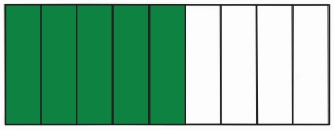
\includegraphics[width=0.5\linewidth]{images/a2.png}
\end{figure}

3. What does 2/7 represent? You can describe it or draw a picture.

4. What fractional number of this set represents cats?

\begin{figure}[h]
    \centering
    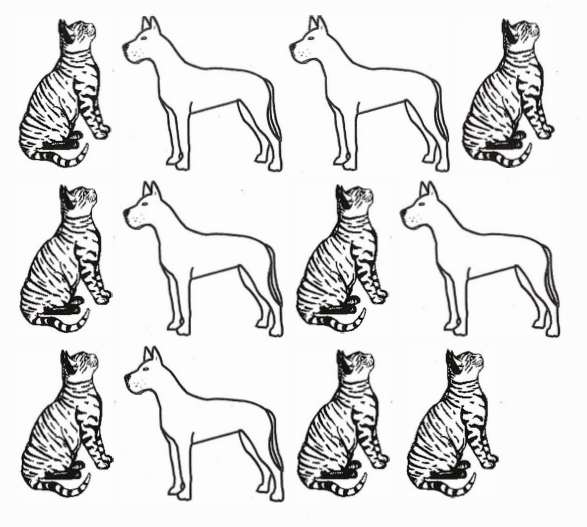
\includegraphics[width=0.5\linewidth]{images/a4.png}
\end{figure}

5. Which shows 2/3 of the square shaded? Please circle one.

\begin{figure}[h]
    \centering
    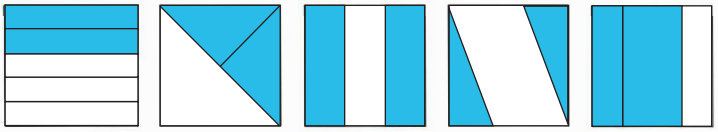
\includegraphics[width=0.5\linewidth]{images/a5.png}
\end{figure}
\clearpage
Order Questions

1. 1/9 or 1/5 Are they equal? \textbf{YES} \textbf{NO} If not which one is smaller?

2. 3/4 or 2/3 Are they equal? \textbf{YES} \textbf{NO} If not which one is larger?

3. 5/3 or 3/5 Are they equal? \textbf{YES} \textbf{NO} If not which one is smaller?

4. Please put the letters (a, b, c) in order from the largest fraction to the smallest fraction.

\begin{figure}[h]
    \centering
    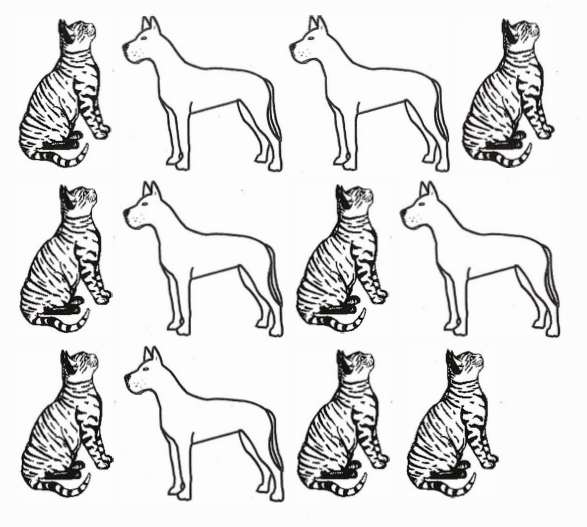
\includegraphics[width=0.5\linewidth]{images/a4.png}
\end{figure}

5. 1/5 3/4 1/2

Please put the fractions in order from the smallest fraction to the largest fraction.
\clearpage
Equivalence Questions

1. Which one of the following fractions is equivalent to 1/3? Please circle one:

2/5 2/9 2/6

2. Which one of the following fractions is equivalent to 2/1? Please circle one:

1/2 3/2 4/2

3. Which one of the following fractions is equivalent to the fraction that shows how much of the circle is shaded? Please circle one.

\begin{figure}[h]
    \centering
    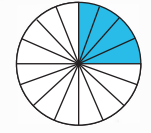
\includegraphics[width=0.2\linewidth]{images/c3.png}
\end{figure}

5/16 1/4 4/8 1/8

4. Please shade the equivalent fraction as show in Rectangle A in Circle A.

\begin{figure}[h]
    \centering
    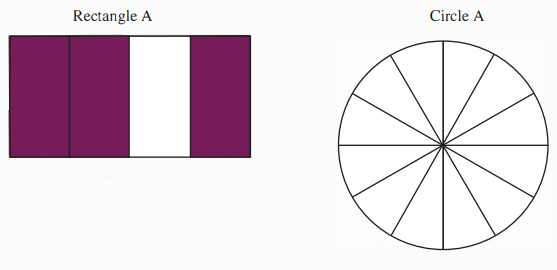
\includegraphics[width=0.5\linewidth]{images/c4.png}
\end{figure}

5. Which one of the following rectangle has the equivalent fraction as Figure A?

\begin{figure}[h]
    \centering
    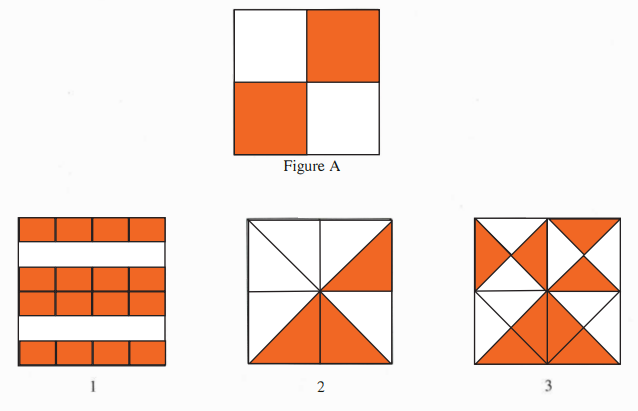
\includegraphics[width=0.5\linewidth]{images/c5.png}
\end{figure}
\end{document}
